Bevor ein erster Prototyp erstellt werden konnte, mussten die richtigen Bauteile ausgewählt werden. Dies Geschah unteranderem anhand der gewonnenen Informationen aus dem Kapitel 2 Vorbereitung. 

\subsection{Mikrocontroller}
Der Infineon XMC 1404\_Q048 gehört zur Familie der ARM Cortex -M0 Prozessoren und ist ein 32~Bit Industrial Mikrocontroller, wird mit 48~MHz externer Clock betrieben. Die Q048 im Namen steht für die Anzahl der Pins. Der interne Timer läuft mit 96~MHz. Die CCU4 des Prozessors bietet ein 2x4 16~Bit Timer. Zudem hat der XMC einen 12~Bit A/D Wandler, welcher für die Analogmessung eine genauere Auflösung bieten kann als ein 8~Bit A/D Wandler. Die Betriebsspannung des Prozessors beträgt 3,3~V. Die Auswahl des Mikrocontrollers wurde getroffen, weil dieser standardmäßig bei Tinkerforge eingesetzt wird und uns für den Prototypen vorgegeben wurde. 


\subsection{Sender}Um eine Trennung zwischen der Mikrocontroller, (3,3~V) und dem Hochsetzsteller (5~V-20~V)zu ermöglichen, benötigte zusätzlich ein weiteres Bauteil. Dafür wurde das IC A5950 (Voll Brücke) ausgewählt. Diese H-Brücke kann eine angeschlossene Last mit der vom Hochsetzstellers erzeugten Spannung versorgen. Deren Frequenz wird über das Signal an dem Pin \glqq Phase \grqq~von dem Prozessor vorgegeben. An den Anschlüssen Out1 und Out2 wird das Ausgangssignal abgegriffen. Für die genaue Beschaltung des ICs siehe Anhang Datenblatt  \glqq Schimatic A5950 \grqq.




\subsection{Hochsetzsteller}
Tinkerforge nutzt schon eine Variante eines Hochsetzstellers auf ihren Platinen. Der Aufbau und die Bauteilauswahl mussten nur auf die variable Ausgangspannungs erweitert werden. Die Standardschaltung, von Tinkerforge, wurde an dem Eingang der Feedbackspannung mit einem Potentiometer (RV1) ergänzt, um die gewünschte variable Spannung zu generieren.\\
Die Ausgangsspannung wird mit den externen Widerständen RV1, R13 und R2 eingestellt (siehe Grundschaltung Datenblatt vom IC LRM62014x, Seite 11). Ein Wert von ca. \(\displaystyle 13,3~k\Omega \) wurde für R2 empfohlen. Mit den Potentiometer (RV1) lässt sich die Ausgangsspannung bei 5~V Eingangsspannung bis 21,5~V einstellen. In der Formel werden die Widerstände RV1 und R13 zum Ersatzwiderstand(Re) zusammengefasst.
\onehalfspacing \\
\[\displaystyle Re=R2*\left(\frac{Vout}{1,23}-1\right) \Rightarrow Vout=\left(\frac{Re}{R2}+1\right)*1,23\] 
\singlespacing
\begin{center}
\begin{minipage}{1\textwidth}
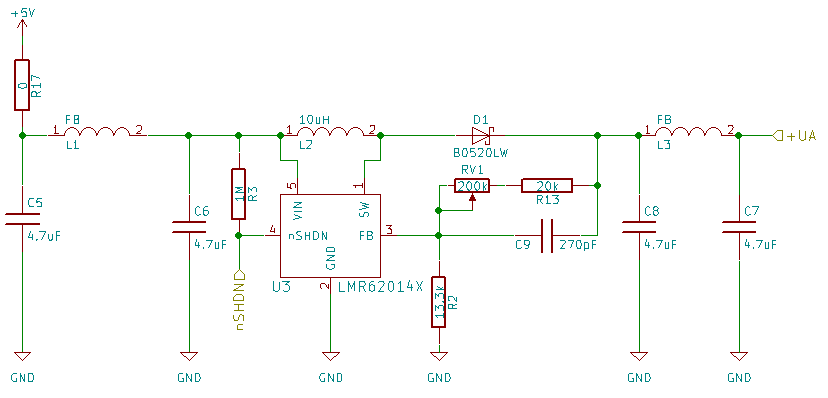
\includegraphics[width=1\textwidth%, draft
]{Abbildungen/Pumpe.png}
\captionof{figure}{Schaltplan des beschalteten Hochsetzstellers}
\label{fig:Hochsetzsteller}
\end{minipage}\\
\end{center}

\subsection{Ultraschallkapsel}%bearbeiten
Für den Prototypen wurden mehrere Kapseln diverser Hersteller bestellt. Dieses geschah um Unterschiede der verschieden preisigen Bauteile zu ermitteln und um festzustellen, welches Preissegment die nötige Qualität für die vorliegende Anwendung erfüllt.


\subsection{Filter}%bearbeiten
Um unerwünschte Signalanteile mit Frequenzen, die unter 40~kHz liegen, zu unterdrücken musste die Filterschaltung mit einem Hochpassfilter (CR Glied) bestehend aus einem Kodensator und einem Widerstand bestückt. Der Widerstand wurde nach der e24 Reihe ausgewählt.
Die Kapazität des Kondensators wurde an die Grenzfrequenz von 40~kHz und den Widerstand angepasst.
\onehalfspacing \\
\[\displaystyle C=\frac{1}{2*pi*fg*R}\Rightarrow\frac{1}{2*pi*40~kHz*100~K\Omega}\approx40~pF \]
\singlespacing
Anhand der Berechnung wurde für den Hochpassfilter ein Kondensator mit \(\displaystyle 39~pF\) genommen.

\subsection{Empfänger}
Die Abbildung \ref{fig:Empfängerschaltung} zeigt die Empfängerschaltung. Durch diese Verschaltung von Operationsverstärkern wird das ankommende sinusförmige Signal verstärkt und in ein digitales Signal umgewandelt. Für die Verstärkung der Amplitude und der Umwandlung des analogen Signals in ein Rechtecksignal mit 40~KHz wurde der das IC TLC272 ausgewählt, weil dieser günstig im Stückpreis ist und die technischen Spezifikationen ausreichend sind. Siehe Datenblatt vom IC TLC272.\\

Für die Verstärkung der Amplitude ist der Operationsverstärker TLC272 U2B als nicht invertierender Verstärker geschaltet.
Für die Umwandlung des analogen Signales in ein digitales wurde der Operationsverstärker TLC272 U2C als Komparator geschaltet. Beim Auftreten von Differenzen zwischen den Eingangssignalen, wechselt der Ausgang des Komparators zwischen Low (0~Volt) auf High (3,3~Volt).\\ Die Referenzspannung (\(\displaystyle Uref)\)  wird durch den Spannungsteiler R9 und R8 bestimmt.
\onehalfspacing \\
\[\displaystyle Uref=\frac{Uges*R9}{R8+R9}\Rightarrow\frac{3,3~V*120~K\Omega}{100~K\Omega+120~K\Omega}=1,8~V \]
\singlespacing
\begin{center}
\begin{minipage}{1\textwidth}
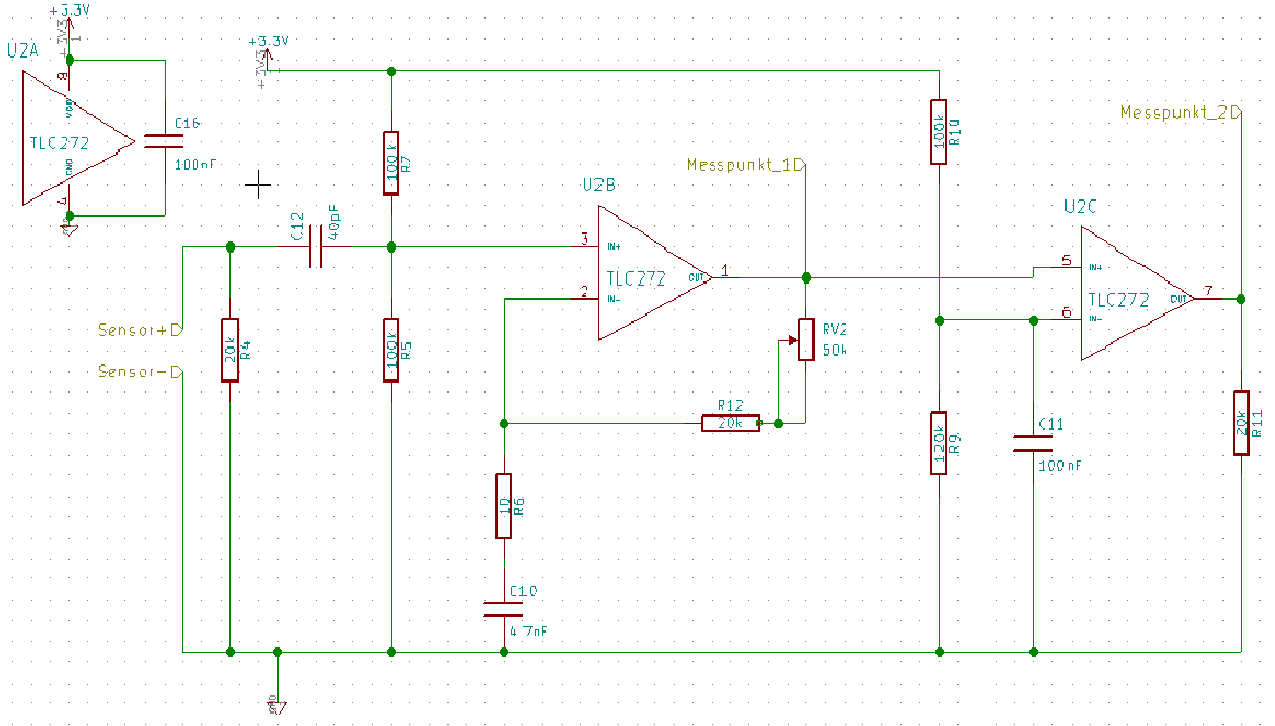
\includegraphics[width=1\textwidth%, draft
]{Abbildungen/Empfaenger.png}
\captionof{figure}{Schaltplan zweier Operationsverstärker mit einer vorgelagerten Filterung als Empfängerschaltung}
\label{fig:Empfaengerschaltung}
\end{minipage}\\
\end{center}

